\documentclass[aspectratio=169]{beamer}
\usepackage[utf8]{inputenc}

% design
\usetheme{CambridgeUS}
\usecolortheme{beaver}
\setbeamertemplate{itemize items}[square]
\usenavigationsymbolstemplate{\beamertemplatenavigationsymbolsempty}
\definecolor{darkred}{rgb}{0.8,0,0}
\setbeamertemplate{enumerate item}{\color{darkred}\insertenumlabel.}
\setbeamertemplate{itemize item}{\color{darkred}$\blacktriangleright$}

% bibliography
%\usepackage[backend=biber, style=authortitle]{biblatex}
\usepackage{natbib}
\usepackage{har2nat}
\bibliographystyle{unsrt}
%\addbibresource{../../smc.bib}
\usepackage{bibentry}
\nobibliography*

% tikz
\usepackage{tikz}
\usetikzlibrary{positioning}

% maths
\usepackage{amsmath}
\usepackage{amssymb}
\usepackage{amsthm}
\theoremstyle{definition}
\newtheorem{defn}{Definition}

% useful math symbols
\newcommand{\PR}{\mathbb{P}}
\newcommand{\E}{\mathbb{E}}
\newcommand{\V}{\operatorname{Var}}
\newcommand{\eqdist}{\overset{d}{=}}
\newcommand{\I}[1]{\mathbb{I}\{#1\}}
\newcommand{\Ntoinfty}{\overset{N\to\infty}{\longrightarrow}}
\newcommand{\limNtoinfty}{\underset{N\to\infty}{\lim}}
\newcommand\indep{\protect\mathpalette{\protect\independenT}{\perp}}
\def\independenT#1#2{\mathrel{\rlap{$#1#2$}\mkern2mu{#1#2}}}

% distributions
\newcommand{\N}{\mathcal{N}}
\newcommand{\Cat}{\operatorname{Categorical}}
\newcommand{\Unif}{\operatorname{Uniform}}
\newcommand{\Mn}{\operatorname{Multinomial}}
\newcommand{\Bin}{\operatorname{Binomial}}

% project-specific commands
\newcommand{\F}{\mathcal{F}_{t-1}}
%\newcommand{\vt}[2][t]{v_{#1}^{(#2)}}
\newcommand{\vt}[1]{v_{#1}}
%\newcommand{\wt}[2][t]{w_{#1}^{(#2)}}
\newcommand{\wt}[1]{w_{#1}}
%\newcommand{\wbar}[2][t]{\bar{w}_{#1}^{(#2)}}
%\newcommand{\vttilde}[2][t]{\tilde{v}_{#1}^{(#2)}}

\title[Resampling in SMC]{Resampling in Sequential Monte Carlo}
\author{Suzie Brown}
\date{12 November 2019} 

\begin{document}
\begin{frame}
\maketitle
\end{frame}


\begin{frame}{Resampling Schemes}{Definition}
%Let $\mathcal{S}_k$ denote the simplex on $k$ elements
%\begin{equation}
%\mathcal{S}_k := \left\{ (x_1, \dots, x_k) : x_i \geq 0, \sum x_i = 1 \right\}
%\end{equation}
%
%We will call a map {\color{darkred}$\wt{1:N} \in \mathcal{S}_N \longrightarrow \vt{1:N} \in \mathbb{N}^N$} a \emph{resampling scheme} if it satisfies the following
%\begin{itemize}
%\item Number of particles is constant: $\sum_{i=1}^N \vt{i}(\wt{1:N}) = N$
%\item Unbiased: $\E[\vt{i} \mid \wt{1:N}] = N\wt{i}$ for all $i$
%\item After resampling, all weights are equal to $\frac{1}{N}$
%\end{itemize}
We will take valid resampling schemes to be those satisfying
\begin{itemize}
\item The total number of particles $N$ remains fixed
\item The particles after resampling are equally weighted
\item The scheme is unbiased: the expected number of offspring of particle $i$ is equal to $N\wt{i}$ for each $i$
\end{itemize}

%%% NOTES
% 1. These conditions can be violated in certain ways without destroying the convergence properties of the SMC algorithm, but in practice such schemes are not used much.
%%%
\end{frame}


\begin{frame}{Multinomial Resampling\footnote{Efron \& Tibshirani (1994) `An introduction to the bootstrap'}}{Definition}
Parental indices $a_i \in \{1,\dots,N\}$:
\begin{equation*}
(a_{i} \mid \wt{1:N}) \overset{iid}{\sim} \Cat(N, \wt{1:N})
\end{equation*}
Offspring numbers $\vt{i} \in \{0,\dots,N\}$ such that $\sum \vt{i} = N$:
\begin{equation*}
(\vt{1:N} \mid \wt{1:N}) \sim \Mn(1:N, \wt{1:N})
\end{equation*}

%%% NOTES
% 1. Weight vectors in Categorical/Multinomial distributions are given up to a constant
% 2. May not be the most efficient way, but one way to sample from the Categorical distribution is by inversion sampling. Useful for comparison with other resampling schemes.
%%%
\end{frame}


\begin{frame}{Multinomial Resampling}{Inversion Sampling}
\begin{center}
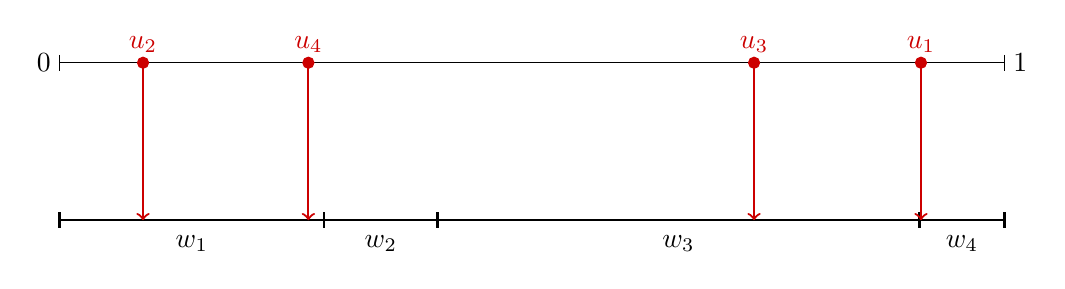
\begin{tikzpicture}
%parallel lines
\draw[thick] (0,0) -- (12,0);
\draw (0,2) -- (12,2);
% tick marks at ends
\draw[thick] (0,0.1) --(0,-0.1);
\draw[thick] (12,0.1) --(12,-0.1);
\draw (0,2.1) --(0,1.9);
\draw (12,2.1) --(12,1.9);
% tick marks indicating weights
\draw[thick] (0.28*12,0.1) --(0.28*12,-0.1);
\draw[thick] (0.4*12,0.1) --(0.4*12,-0.1);
\draw[thick] (0.91*12,0.1) --(0.91*12,-0.1);
% weight labels
\node at (0.28*6,-0.3) {$w_1$};
\node at (0.28*12+0.12*6,-0.3) {$w_2$};
\node at (0.4*12+0.51*6.,-0.3) {$w_3$};
\node at (0.91*12+0.09*6,-0.3) {$w_4$};
% endpoint labels
\node at (-0.2,2) {$0$};
\node at (12.2,2) {$1$};
\pause
% uniform points
\filldraw[darkred] (10.94,2) circle (2pt) node[above] {$u_1$};
\filldraw[darkred] (1.06,2) circle (2pt) node[above] {$u_2$};
\filldraw[darkred] (8.82,2) circle (2pt) node[above] {$u_3$};
\filldraw[darkred] (3.16,2) circle (2pt) node[above] {$u_4$};
\pause
% arrows from random points
\draw[thick, darkred, ->] (10.94,2) -- (10.94,0);
\draw[thick, darkred, ->] (1.06,2) -- (1.06,0);
\draw[thick, darkred, ->] (8.82,2) -- (8.82,0);
\draw[thick, darkred, ->] (3.16,2) -- (3.16,0);
\end{tikzpicture}
\end{center}

%%% NOTES
% 1. Use the weights to partition [0,1]
% 2. Draw N i.i.d. Uniform[0,1] samples
% 3. Number of points falling in each interval gives the offspring counts (2,0,1,1)
%%%
\end{frame}


\begin{frame}{Residual Resampling\footnote{Liu \& Chen (1998) `Sequential Monte Carlo methods for dynamic systems'}\textsuperscript{,}\footnote{Whitley (1994) `A genetic algorithm tutorial'}}{Definition}
\begin{enumerate}
\item Deterministically assign $\lfloor N \wt{i} \rfloor$ offspring to particle $i$; i=1,\dots, N
\item There are $R := N- \sum_{i=1}^N \lfloor N \wt{i} \rfloor$ offspring  still to be assigned
\item Assign these randomly according to the residual weights $r_i := \frac{1}{R} (N\wt{i} - \lfloor N\wt{i} \rfloor)$
\end{enumerate}

%%% NOTES
% 1. The deterministic part means high-weight (>1/N) particles are guaranteed to survive
% 2. The random part can be done in various ways e.g. multinomial, stratified
%%%
\end{frame}


\begin{frame}{Residual Resampling}{Definition}
If residuals are assigned using multinomial resampling, offspring counts are distributed
\begin{equation*}
\vt{1:N} \eqdist \lfloor N \wt{1:N} \rfloor +  \Mn(R, r_{1:N})
\end{equation*}
\end{frame}


\begin{frame}{Residual Resampling}{Illustration}
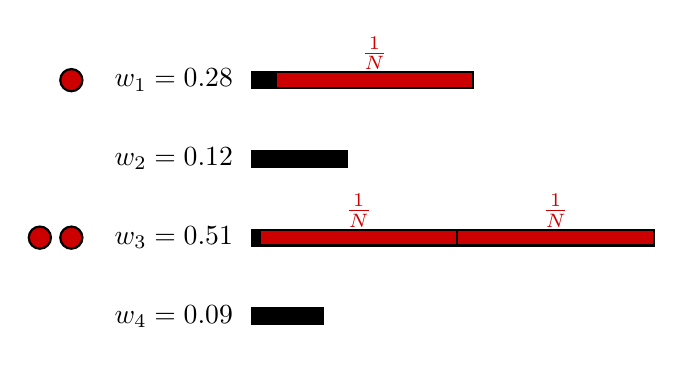
\begin{tikzpicture}
\node at (0,0) {$w_1=0.28$};
\node at (0,-1) {$w_2=0.12$};
\node at (0,-2) {$w_3=0.51$};
\node at (0,-3) {$w_4=0.09$};
\draw[thick, fill=black] (1,0.1) rectangle (1+0.28*10,-0.1);
\draw[thick, fill=black] (1,0.1-1) rectangle (1+0.12*10,-0.1-1);
\draw[thick, fill=black] (1,0.1-2) rectangle (1+0.51*10,-0.1-2);
\draw[thick, fill=black] (1,0.1-3) rectangle (1+0.09*10,-0.1-3);
\pause
\draw[thick,fill=darkred] (1+0.03*10,0.1) rectangle
node[above, color=darkred] {$\frac{1}{N}$} (1+0.28*10,-0.1);
\draw[thick, fill=darkred] (1+0.01*10,0.1-2) rectangle 
node[above, color=darkred] {$\frac{1}{N}$} (1+0.26*10,-0.1-2);
\draw[thick, fill=darkred] (1+0.26*10,0.1-2) rectangle 
node[above, color=darkred] {$\frac{1}{N}$} (1+0.51*10,-0.1-2);
\pause
\draw[thick, fill=darkred] (-1.3,0) circle (4pt);
\draw[thick, fill=darkred] (-1.3,-2) circle (4pt);
\draw[thick, fill=darkred] (-1.7,-2) circle (4pt);
\end{tikzpicture}
\end{frame}


\begin{frame}{Residual Resampling}{Illustration}
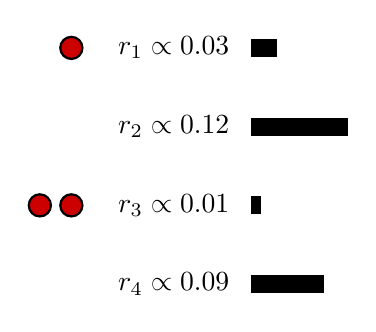
\begin{tikzpicture}
\draw[thick, fill=darkred] (-1.3,0) circle (4pt);
\draw[thick, fill=darkred] (-1.3,-2) circle (4pt);
\draw[thick, fill=darkred] (-1.7,-2) circle (4pt);
\node at (0,0) {$r_1 \propto 0.03$};
\node at (0,-1) {$r_2 \propto 0.12$};
\node at (0,-2) {$r_3 \propto 0.01$};
\node at (0,-3) {$r_4 \propto 0.09$};
\draw[thick, fill=black] (1,0.1) rectangle (1+0.03*10,-0.1);
\draw[thick, fill=black] (1,0.1-1) rectangle (1+0.12*10,-0.1-1);
\draw[thick, fill=black] (1,0.1-2) rectangle (1+0.01*10,-0.1-2);
\draw[thick, fill=black] (1,0.1-3) rectangle (1+0.09*10,-0.1-3);
\end{tikzpicture}
\end{frame}


\begin{frame}{Residual Resampling}{Illustration}
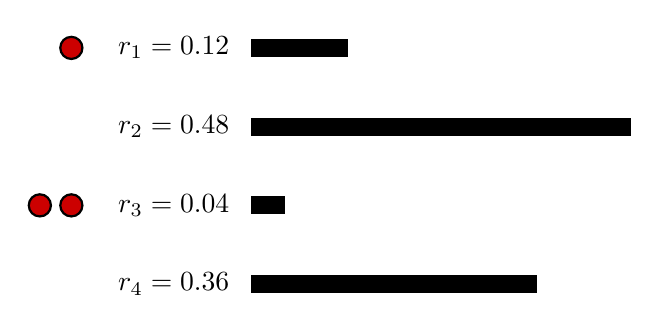
\begin{tikzpicture}
\draw[thick, fill=darkred] (-1.3,0) circle (4pt);
\draw[thick, fill=darkred] (-1.3,-2) circle (4pt);
\draw[thick, fill=darkred] (-1.7,-2) circle (4pt);
\node at (0,0) {$r_1 = 0.12$};
\node at (0,-1) {$r_2 = 0.48$};
\node at (0,-2) {$r_3 = 0.04$};
\node at (0,-3) {$r_4 = 0.36$};
\draw[thick, fill=black] (1,0.1) rectangle (1+0.03*40,-0.1);
\draw[thick, fill=black] (1,0.1-1) rectangle (1+0.12*40,-0.1-1);
\draw[thick, fill=black] (1,0.1-2) rectangle (1+0.01*40,-0.1-2);
\draw[thick, fill=black] (1,0.1-3) rectangle (1+0.09*40,-0.1-3);
\end{tikzpicture}
\end{frame}


\begin{frame}{Stratified Resampling\footnote{Kitagawa (1996) `Monte Carlo filter and smoother for non-Gaussian nonlinear state space models'}}{Definition}
Draw uniformly from each stratified interval
\begin{equation*}
U_i \sim \Unif \left(\frac{i-1}{N}, \frac{i}{N} \right); \qquad i=1,\dots,N
\end{equation*}
and determine the parental indices by inversion
\begin{equation*}
a_i = \inf\left\{ k: \sum_{j=1}^{k} \wt{j} \geq U_i \right\}
\end{equation*}
\end{frame}


\begin{frame}{Stratified Resampling}{Inversion Sampling}
\begin{center}
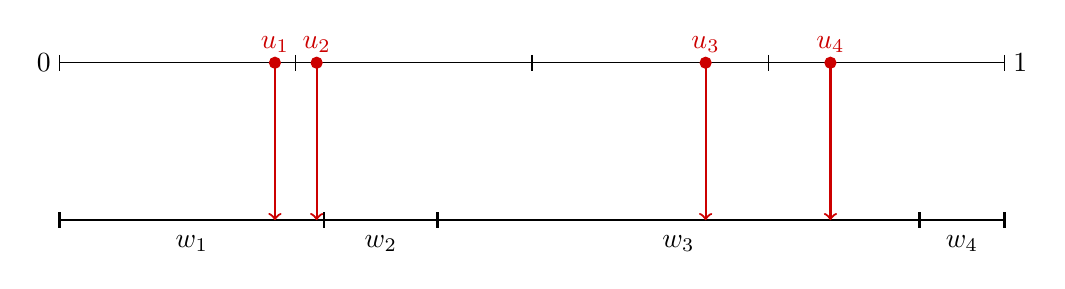
\begin{tikzpicture}
%parallel lines
\draw[thick] (0,0) -- (12,0);
\draw (0,2) -- (12,2);
% tick marks at ends
\draw[thick] (0,0.1) --(0,-0.1);
\draw[thick] (12,0.1) --(12,-0.1);
\draw (0,2.1) --(0,1.9);
\draw (12,2.1) --(12,1.9);
% tick marks indicating sampling intervals:
\draw (3,2.1) --(3,1.9);
\draw (6,2.1) --(6,1.9);
\draw (9,2.1) --(9,1.9);
% tick marks indicating weights
\draw[thick] (0.28*12,0.1) --(0.28*12,-0.1);
\draw[thick] (0.4*12,0.1) --(0.4*12,-0.1);
\draw[thick] (0.91*12,0.1) --(0.91*12,-0.1);
% weight labels
\node at (0.28*6,-0.3) {$w_1$};
\node at (0.28*12+0.12*6,-0.3) {$w_2$};
\node at (0.4*12+0.51*6.,-0.3) {$w_3$};
\node at (0.91*12+0.09*6,-0.3) {$w_4$};
% endpoint labels
\node at (-0.2,2) {$0$};
\node at (12.2,2) {$1$};
\pause
% stratified points
\filldraw[darkred] (2.735,2) circle (2pt) node[above] {$u_1$};
\filldraw[darkred] (3.265,2) circle (2pt) node[above] {$u_2$};
\filldraw[darkred] (8.205,2) circle (2pt) node[above] {$u_3$};
\filldraw[darkred] (9.79,2) circle (2pt) node[above] {$u_4$};
% arrows from random points
\draw[thick, darkred, ->] (2.735,2) -- (2.735,0);
\draw[thick, darkred, ->] (3.265,2) -- (3.265,0);
\draw[thick, darkred, ->] (8.205,2) -- (8.205,0);
\draw[thick, darkred, ->] (9.79,2) -- (9.79,0);
\end{tikzpicture}
\end{center}

%%% NOTES
% 1. Like in Multinomial resampling, but this time the Uniform random numbers are stratified, so there is exactly one in each interval [(i-1)/N, i/N]; i=1,...,N.
% 2. Here I used the same U[0,1] seeds as in m/n but transformed them to the stratified intervals.
% 3. In this example, we get offspring counts (2,0,2,0).
%%%
\end{frame}


\begin{frame}{Systematic Resampling\footnote{Carpenter, Clifford \& Fearnhead (1999) `Improved particle filter for nonlinear problems'}\textsuperscript{,}\footnote{Whitley (1994) `A genetic algorithm tutorial'}}{Definition}
Draw uniformly from $[0, \frac{1}{N}]$, and add multiples of $\frac{1}{N}$
\begin{equation*}
U_1 \sim \Unif \left(0, \frac{1}{N} \right)
\end{equation*}
\begin{equation*}
U_i = U_1 + \frac{i-1}{N}; \qquad i=2,\dots,N
\end{equation*}
and determine the parental indices by inversion
\begin{equation*}
a_i = \inf\left\{ k: \sum_{j=1}^{k} \wt{j} \geq U_i \right\}
\end{equation*}
\end{frame}


\begin{frame}{Systematic Resampling}{Inversion Sampling}
\begin{center}
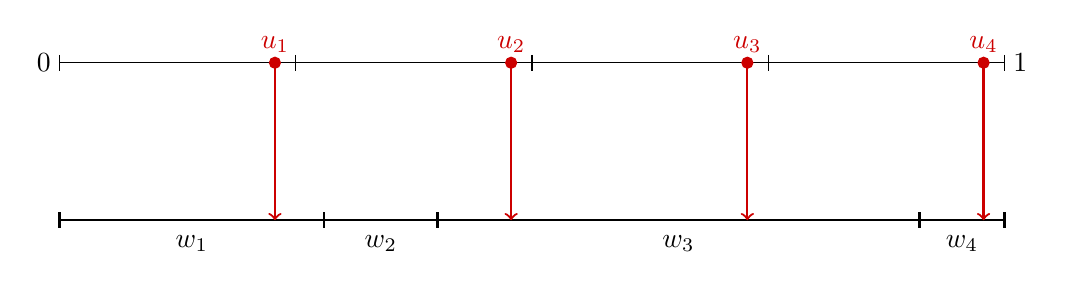
\begin{tikzpicture}
%parallel lines
\draw[thick] (0,0) -- (12,0);
\draw (0,2) -- (12,2);
% tick marks at ends
\draw[thick] (0,0.1) --(0,-0.1);
\draw[thick] (12,0.1) --(12,-0.1);
\draw (0,2.1) --(0,1.9);
\draw (12,2.1) --(12,1.9);
% tick marks indicating sampling intervals:
\draw (3,2.1) --(3,1.9);
\draw (6,2.1) --(6,1.9);
\draw (9,2.1) --(9,1.9);
% tick marks indicating weights
\draw[thick] (0.28*12,0.1) --(0.28*12,-0.1);
\draw[thick] (0.4*12,0.1) --(0.4*12,-0.1);
\draw[thick] (0.91*12,0.1) --(0.91*12,-0.1);
% weight labels
\node at (0.28*6,-0.3) {$w_1$};
\node at (0.28*12+0.12*6,-0.3) {$w_2$};
\node at (0.4*12+0.51*6.,-0.3) {$w_3$};
\node at (0.91*12+0.09*6,-0.3) {$w_4$};
% endpoint labels
\node at (-0.2,2) {$0$};
\node at (12.2,2) {$1$};
\pause
% systematic points
\filldraw[darkred] (2.735,2) circle (2pt) node[above] {$u_1$};
\filldraw[darkred] (5.735,2) circle (2pt) node[above] {$u_2$};
\filldraw[darkred] (8.735,2) circle (2pt) node[above] {$u_3$};
\filldraw[darkred] (11.735,2) circle (2pt) node[above] {$u_4$};
% arrows from random points
\draw[thick, darkred, ->] (2.735,2) -- (2.735,0);
\draw[thick, darkred, ->] (5.735,2) -- (5.735,0);
\draw[thick, darkred, ->] (8.735,2) -- (8.735,0);
\draw[thick, darkred, ->] (11.735,2) -- (11.735,0);
\end{tikzpicture}
\end{center}

%%% NOTES
% 1. Similar to stratified resampling, we ensure exactly one uniform point in each interval
% 2. Here we use just one random seed which is transformed for each interval: u_1 in [0,1/N], then the rest obtained by adding multiples of 1/N.
% 3. In this case the offspring counts are (1,0,2,1).
\end{frame}



\begin{frame}[allowframebreaks]{References}

{\small 
%\printbibliography
%\bibliography{../../smc.bib}
%%% Add references by hand ?
}
\end{frame}
\end{document}